\section{Restoration Results}
\label{sec:restoration-results}

\begin{figure*}[!t]
\centering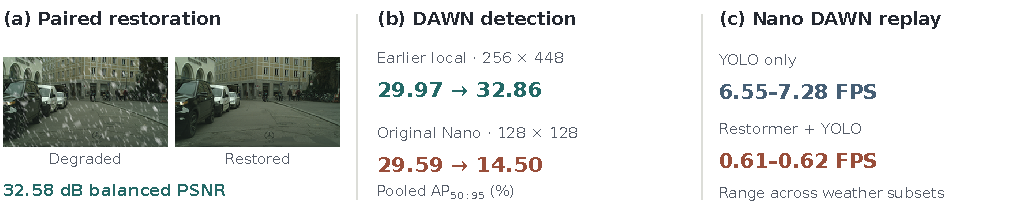
\includegraphics[width=\textwidth]{figures/results_overview.pdf}
\caption{Restoration, detection, and Nano replay. \textbf{(a)} A held-out snow example and balanced PSNR. \textbf{(b)} Pooled DAWN AP$_{50:95}$ in the earlier local and on-device evaluations. Each comparison uses its own geometry and scoring path. \textbf{(c)} Measured throughput ranges across the labelled Nano replay subsets.}
\label{fig:system}
\end{figure*}


\begin{figure*}[!t]
\centering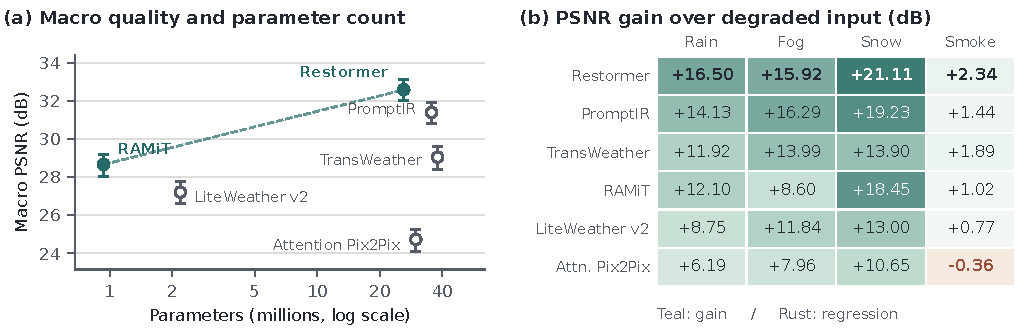
\includegraphics[width=\textwidth]{figures/benchmark_tradeoffs.pdf}
\caption{Performance across six trained systems. \textbf{(a)} Macro PSNR versus parameter count. Bars are 95\% cluster-bootstrap intervals conditional on the fixed checkpoints and test groups. The dashed segment connects the measured quality--size frontier. \textbf{(b)} Weather-balanced PSNR gain over the degraded input. Smoke has the smallest gains for all six systems.}
\label{fig:size}
\end{figure*}

\begin{table*}[!t]
\centering\small\setlength{\tabcolsep}{6.5pt}
\caption{Native-resolution test results on 2,334 pairs. Weather columns report PSNR in dB. Macro metrics follow Eq.~\ref{eq:metric}. Bold marks the best measured values. Shading identifies the retained Restormer.}
\label{tab:six}
\begin{tabular}{@{}lrrrrrrrr@{}}\toprule
\rowcolor{aegishead}
Model & Params (M)& Epoch & Rain & Fog & Snow & Smoke & Macro PSNR & Macro SSIM\\\midrule
\rowcolor{aegisbest}
Restormer &26.127&51&\textbf{38.77}&31.51&\textbf{39.51}&\textbf{20.55}&\textbf{32.58}&\textbf{0.9297}\\
PromptIR &35.592&50&36.40&\textbf{31.88}&37.63&19.65&31.39&0.9182\\
TransWeather &38.052&58&34.19&29.58&32.31&20.10&29.04&0.9000\\
RAMiT &\textbf{0.935}&45&34.37&24.19&36.85&19.23&28.66&0.8995\\
LiteWeather v2 &2.189&59&31.02&27.42&31.40&18.98&27.21&0.8644\\
Attention Pix2Pix &29.855&59&28.46&23.55&29.05&17.85&24.73&0.8201\\\bottomrule
\end{tabular}
\end{table*}

\paragraph{Quality and model size favor different systems.}
Restormer gains 13.97 dB over degraded inputs and leads three of four weather columns (Tab.~\ref{tab:six}). PromptIR leads fog PSNR by 0.38 dB. RAMiT uses about $28\times$ fewer parameters than Restormer, with a 3.92 dB macro gap (Fig.~\ref{fig:size}a). LiteWeather v2 closes part of the fog gap relative to RAMiT, but trails it on macro PSNR. The device trials in Sec.~\ref{sec:edge} address execution.

\paragraph{Smoke is the clearest remaining weakness.}
Restormer's smoke gain is 2.34 dB, versus 15.92--21.11 dB on the other weathers (Fig.~\ref{fig:size}b). Of 342 smoke images, 27 lose PSNR and 37 lose SSIM relative to the raw input. Attention Pix2Pix also regresses on balanced smoke PSNR and SSIM. The qualitative panels (Fig.~\ref{fig:qual}) show streak and snow removal, increased contrast in haze, and residual smoke compared with the target. Six smoke backgrounds limit generalization from these outcomes.

\begin{figure*}[!t]
\centering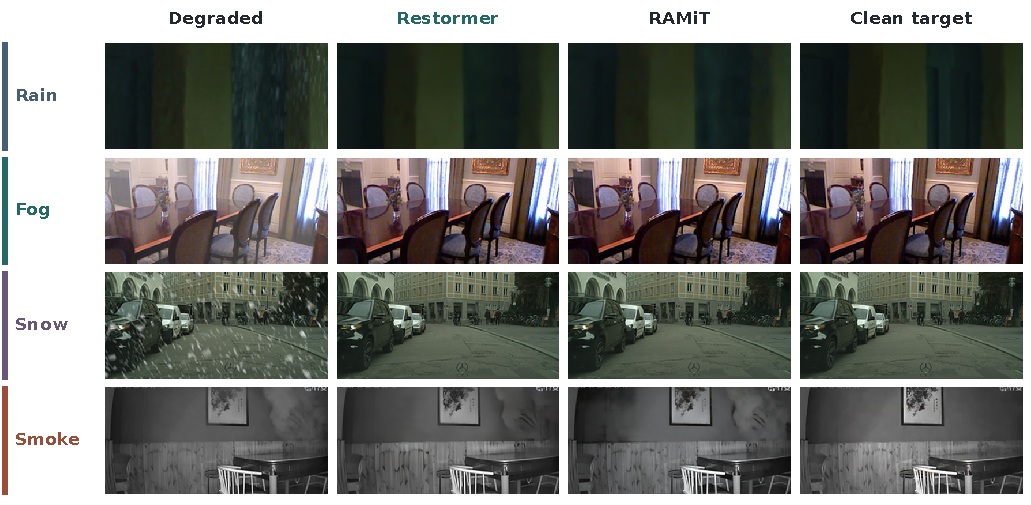
\includegraphics[width=\textwidth]{figures/weather_examples.pdf}
\caption{Same-scene comparison across rain, fog, snow, and smoke. All columns within a row show the same display crop. Source examples were fixed by sample-ID hash before inspecting model scores. These saved predictions use native-resolution CPU FP32. The benchmark in Tab.~\ref{tab:six} uses BF16 over all test pairs.}
\label{fig:qual}
\end{figure*}

\section{Continuation with Matched Training}
\label{sec:jointresults}

\begin{figure*}[!t]
\centering
\begin{minipage}[c]{.49\textwidth}
\centering
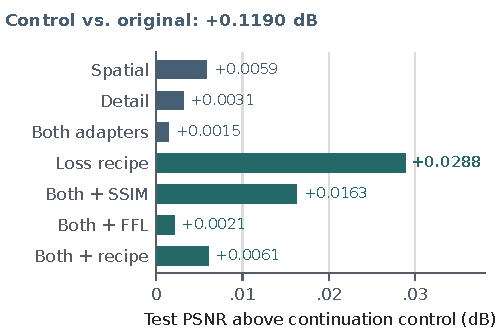
\includegraphics[width=\linewidth]{figures/continuation_gains.pdf}
\end{minipage}\hfill
\begin{minipage}[c]{.48\textwidth}
\centering\small\setlength{\tabcolsep}{4.5pt}
\begin{tabular}{@{}lrr@{}}\toprule
\rowcolor{aegishead}
Model / arm & PSNR (dB) & SSIM\\\midrule
Original epoch 51 &32.5831&0.929690\\
Continuation control &32.7020&0.930786\\
Spatial &32.7079&0.930815\\
Detail &32.7052&0.930799\\
Both adapters &32.7035&0.930783\\
Loss recipe only &\textbf{32.7308}&0.931661\\
Both + SSIM &32.7183&\textbf{0.931719}\\
Both + FFL &32.7042&0.930598\\
Both + recipe &32.7081&0.931440\\\bottomrule
\end{tabular}
\end{minipage}
\caption{Eight-arm continuation results. The plot shows test PSNR gains relative to the matched control. Blue denotes adapter-only arms. Teal denotes loss changes. The table gives test values, with observed maxima in bold. Validation retains the original epoch-51 checkpoint.}
\label{fig:joint}
\end{figure*}

The matched control adds 0.1190 dB over epoch 51. Spatial, detail, and combined adapters add at most 0.0059 dB above it. The largest test gain, 0.0288 dB, comes from changing the loss on the unchanged architecture (Fig.~\ref{fig:joint}). No arm meets the validation replacement rule, so we retain epoch 51 before testing. Further seeds are needed to resolve gains of this size.

\section{Detection Across Operating Points}
\label{sec:dawn}

\begin{figure*}[!t]
\centering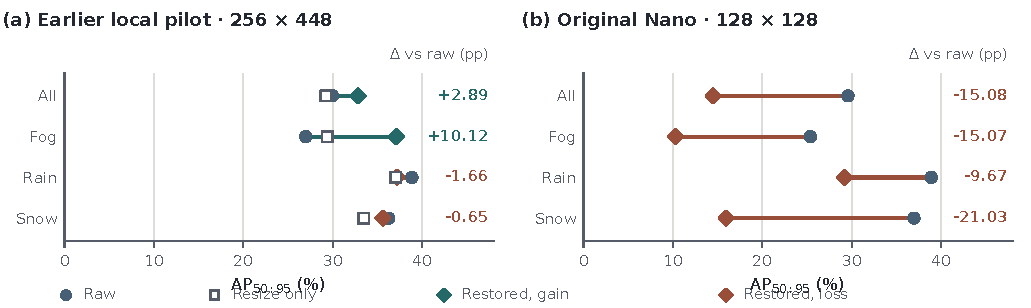
\includegraphics[width=\textwidth]{figures/dawn_operating_points.pdf}
\caption{Labelled DAWN detection in the earlier local pilot and the Nano benchmark. The local comparison includes a $256\times448$ resize-only view. The Nano comparison evaluates the complete $128\times128$ cascade. Both use 72 images, 24 per weather. Signed values show restored-minus-raw AP in percentage points within each evaluation.}
\label{fig:det}
\end{figure*}

\begin{figure*}[!t]
\centering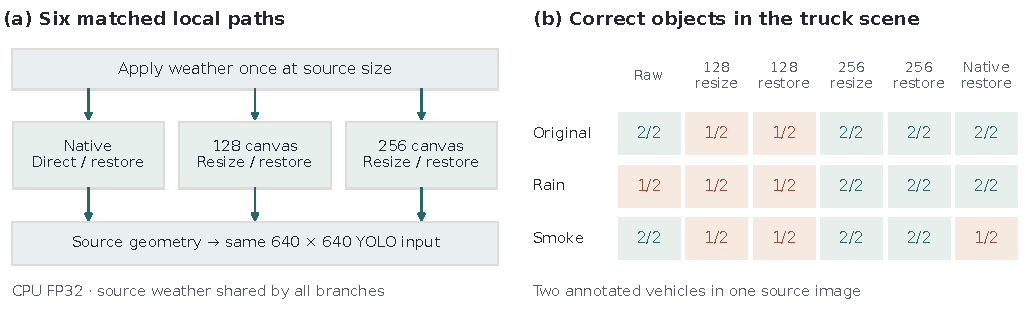
\includegraphics[width=\textwidth]{figures/controlled_resolution.pdf}
\caption{Matched local resolution diagnostic. \textbf{(a)} The same degraded source enters all branches. Native restoration only pads and crops. Each branch maps to the source geometry and uses the same detector preprocessing. \textbf{(b)} Correct detections among two annotated vehicles in one DAWN scene. Under rain, the 256 resize-only view already recovers both vehicles. Native restoration gains a match in rain and loses one in smoke.}
\label{fig:resolution}
\end{figure*}

\paragraph{Earlier local pilot.}
DAWN~\cite{Kenk_2020_DAWN} supplies real-weather road-object labels. The earlier local evaluation compares raw, resize-only, and restored views on 72 labelled images with one frozen COCO-pretrained YOLOv8n. The two transformed views use a $256\times448$ canvas and return to original geometry before $640\times640$ detector preprocessing. Pooled AP$_{50:95}$ rises from 29.97\% raw to 32.86\% restored, with the resize-only control at 29.25\%. Fog improves by 10.12 points against raw input. Rain and snow decline by 1.66 and 0.65 points (Fig.~\ref{fig:det}a).

\paragraph{Labelled Nano benchmark.}
The measured Nano evaluation has 72 images and 541 labelled objects across fog, rain, and snow. The $128\times128$ Restormer path returns to source geometry before the same YOLO engine. Pooled AP$_{50:95}$ falls from 29.59\% to 14.50\%, a 15.08-point loss (Fig.~\ref{fig:det}b). At confidence 0.25 and IoU 0.50, matched objects fall from 270 to 110, and misses rise from 271 to 431. AP uses detections from confidence 0.001, class-aware NMS at 0.7, and at most 100 detections per image. Geometry, runtime, and scoring differ from the earlier local pilot. The measured drop pertains to the complete Nano cascade.

\paragraph{Matched resolution controls.}
In the separate local FP32 diagnostic, each source receives the same synthetic degradation before any branch resizes it. We compare direct detection, resize-only and restored views at 128 and 256, and native restoration (Fig.~\ref{fig:resolution}). The 128 resize-only path misses the truck in the original hazy scene. The 256 resize-only path recovers it under rain, with the 256 restorer adding zero matched objects over the resize control in the tested weather variants. Native restoration recovers the rainy truck and misses the smoky truck. These cases repeat five annotated objects across weather conditions. A third camera scene contributes prediction counts only. Supplementary Appendix~D gives the full diagnostic and timing scopes.
